%\documentclass[a4paper,UKenglish]{lipics}
\documentclass[11pt]{article}
\usepackage{microtype}%if unwanted, comment out or use option "draft"
\usepackage{xspace}
\usepackage{bbm}
%\usepackage{times}
\usepackage{graphicx}
%\usepackage{amsmath,amssymb,amsthm,mathtools}
\usepackage{amsmath,amssymb,amsthm}

\usepackage{paralist}
\usepackage{bm}
\usepackage{xspace}
\usepackage{url}
\usepackage{fullpage, prettyref}
\usepackage{boxedminipage}
\usepackage{wrapfig}
\usepackage{ifthen}
\usepackage{color}
\usepackage{xcolor}
%\usepackage[noend]{algorithmic}
%\usepackage{algorithmicx}
%\usepackage[noend]{algcompatible}
\usepackage{algpseudocode}

\usepackage{algorithm}
\usepackage{fullpage}
\usepackage{hyperref}
\usepackage[compact]{titlesec}
\usepackage{cleveref}
\usepackage{nicefrac}

\usepackage[bottom=1in,top=1in,left=1in,right=1in]{geometry}
\makeatletter
 \setlength{\parindent}{0pt}
 \addtolength{\partopsep}{-2mm}
 \setlength{\parskip}{5pt plus 1pt}
 %\addtolength{\theorempreskipamount}{-1mm}
 %\addtolength{\theorempostskipamount}{-1mm}
 \addtolength{\abovedisplayskip}{-3mm}
 %\addtolength{\belowcaptionskip}{-6mm}
 % \addtolength{\textheight}{20pt}
 %\addtolength{\footskip}{-20pt}
\makeatother

\usepackage{framed}
\renewenvironment{leftbar}[1][\hsize]
{%
    \def\FrameCommand
    {%
        {\color{gray}\vrule width 4pt}%
        \hspace{1pt}%must no space.
        \fboxsep=\FrameSep\colorbox{gray!20}%
    }%
    \MakeFramed{\hsize#1\advance\hsize-\width\FrameRestore}%
}
{\endMakeFramed}

% For restating theorems in appendix
\usepackage{thmtools}
\usepackage{thm-restate}
\declaretheorem[numberwithin=section]{theorem}
\declaretheorem[sibling=theorem]{lemma}
\declaretheorem[sibling=theorem]{claim}
\declaretheorem[sibling=theorem]{corollary}
%\newtheorem{theorem}{Theorem}[section]
%\newtheorem{conjecture}[theorem]{Conjecture}
%\newtheorem{lemma}[theorem]{Lemma}
%\newtheorem{claim}[theorem]{Claim}
%\newtheorem{corollary}[theorem]{Corollary}
%\newtheorem{definition}[theorem]{Definition}
\newtheorem{problem}[theorem]{Problem}
\newtheorem{definition}[theorem]{Definition}
\crefname{claim}{claim}{claims}

%\newtheorem{fact}[theorem]{Fact}
%\newtheorem{example}[theorem]{Example}
%\newtheorem{assumption}[theorem]{Assumption}
%\newtheorem{observation}[theorem]{Observation}
%\newtheorem{remark}[theorem]{Remark}

%\newcommand{\opt}{{\tt opt}\xspace}

\newcommand{\ex}{{\mathbb E}}
\newcommand{\pr}{{\mathbb P}}

\usepackage[colorinlistoftodos,textsize=tiny,textwidth=2cm,color=red!25!white,obeyFinal]{todonotes}
\newcommand{\nnote}[1]{\todo[color=blue!25!white]{N: #1}\xspace}
\newcommand{\dnote}[1]{\todo[color=green!25!white]{D: #1}\xspace}
\newcommand{\rnote}[1]{\todo[color=red!25!white]{R: #1}\xspace}

%\newcommand{\comment}[1]{\textit {\em \color{red} \footnotesize *}\marginpar{\tiny{\color{blue} #1}}}
% \renewcommand{\comment}[1]{\textit {\em \color{blue} \footnotesize[#1]}\marginpar{\tiny\textsc{\color{blue} To Do!}}}
% \newcommand{\mcomment}[1]{\textbf {\em \color{red} \footnotesize[#1]}\marginpar{\tiny\textsc{\color{red} PLEASE CHECK}}}

\newcommand{\ignore}[1]{}

%\usepackage{cleveref}


%\bibliographystyle{plain}% the recommended bibstyle

\newcommand{\nukc}{{\sf NUkC}\xspace}
\newcommand{\kcwo}{{\sf kCwO}\xspace}
\newcommand{\rmfc}{{\sf RMFC-T}\xspace}
\newcommand{\Itree}{\ensuremath{{\cal I}_T}\xspace}
\newcommand{\I}{\ensuremath{{\cal I}}\xspace}
\newcommand{\treepath}{\ensuremath{\sf treePath}\xspace}
\newcommand{\cov}{\ensuremath{{\sf Cov}}\xspace}
\newcommand{\sse}{\ensuremath{\subseteq}\xspace}

%\newtheorem{claim}{Claim}

\newcommand{\cA}{{\cal A}}
\newcommand{\cB}{\mathcal{B}}
\newcommand{\cC}{{\cal C}}
\newcommand{\cD}{\mathcal{D}}
\newcommand{\cE}{{\cal E}}
\newcommand{\cF}{\mathcal{F}}
\newcommand{\cG}{\mathcal{G}}
\newcommand{\cH}{{\cal H}}
\newcommand{\cI}{{\cal I}}
\newcommand{\cJ}{{\cal J}}
\newcommand{\cL}{{\cal L}}
\newcommand{\cM}{{\cal M}}
\newcommand{\cP}{\mathcal{P}}
\newcommand{\cQ}{\mathcal{Q}}
\newcommand{\cR}{{\cal R}}
\newcommand{\cS}{\mathcal{S}}
\newcommand{\cT}{{\cal T}}
\newcommand{\cU}{{\cal U}}
\newcommand{\cV}{{\cal V}}
\newcommand{\cX}{{\cal X}}


%\DeclareMathOperator*{\argmax}{arg\,max}


\newcommand{\R}{\mathbb R}
\newcommand{\N}{\mathbb N}
\newcommand{\F}{\mathbb F}
\newcommand{\Z}{{\mathbb Z}}
\newcommand{\eps}{\varepsilon}
\newcommand{\lam}{\lambda}
\newcommand{\sgn}{\mathrm{sgn}}


\newcommand{\poly}{\mathrm{poly}}
\newcommand{\polylog}{\mathrm{polylog}}
\newcommand{\polyloglog}{\mathrm{\poly\log\log}}
\newcommand{\littlesum}{\mathop{{\textstyle \sum}}}
\newcommand{\half}{{\textstyle \frac12}}
\newcommand{\la}{\langle}
\newcommand{\ra}{\rangle}
\newcommand{\wh}{\widehat}
\newcommand{\wt}{\widetilde}
\newcommand{\calE}{{\cal E}}
\newcommand{\calL}{{\cal L}}
\newcommand{\calF}{{\cal F}}
\newcommand{\calW}{{\cal W}}
\newcommand{\calH}{{\cal H}}
\newcommand{\calN}{{\cal N}}
\newcommand{\calO}{{\cal O}}
\newcommand{\calP}{{\cal P}}
\newcommand{\calV}{{\cal V}}
\newcommand{\calS}{{\cal S}}
\newcommand{\calT}{{\cal T}}
\newcommand{\calD}{{\cal D}}
\newcommand{\calC}{{\cal C}}
\newcommand{\calX}{{\cal X}}
\newcommand{\calY}{{\cal Y}}
\newcommand{\calZ}{{\cal Z}}
\newcommand{\calA}{{\cal A}}
\newcommand{\calB}{{\cal B}}
\newcommand{\calG}{{\cal G}}
\newcommand{\calI}{{\cal I}}
\newcommand{\calJ}{{\cal J}}
\newcommand{\calR}{{\cal R}}
\newcommand{\calK}{{\cal K}}
\newcommand{\calU}{{\cal U}}
\newcommand{\barx}{\overline{x}}
\newcommand{\bary}{\overline{y}}

\newcommand{\ba}{\boldsymbol{a}}
\newcommand{\bb}{\boldsymbol{b}}
\newcommand{\bp}{\boldsymbol{p}}
\newcommand{\bt}{\boldsymbol{t}}
\newcommand{\bv}{\boldsymbol{v}}
\newcommand{\bx}{\boldsymbol{x}}
\newcommand{\by}{\boldsymbol{y}}
\newcommand{\bz}{\boldsymbol{z}}
\newcommand{\br}{\boldsymbol{r}}
\newcommand{\bh}{\boldsymbol{h}}

\newcommand{\bA}{\boldsymbol{A}}
\newcommand{\bD}{\boldsymbol{D}}
\newcommand{\bG}{\boldsymbol{G}}

\newcommand{\bR}{\boldsymbol{R}}
\newcommand{\bS}{\boldsymbol{S}}
\newcommand{\bX}{\boldsymbol{X}}
\newcommand{\bY}{\boldsymbol{Y}}
\newcommand{\bZ}{\boldsymbol{Z}}

\newcommand{\NN}{\mathbb{N}}
\newcommand{\RR}{\mathbb{R}}

\newcommand{\abs}[1]{\left\lvert #1 \right\rvert}
\newcommand{\norm}[1]{\left\lVert #1 \right\rVert}
\newcommand{\ceil}[1]{\lceil#1\rceil}
\newcommand{\Exp}{\EX}
\newcommand{\floor}[1]{\lfloor#1\rfloor}

\newcommand{\EX}{\hbox{\bf E}}
\newcommand{\prob}{{\rm Prob}}

\newcommand{\gset}{Y}
\newcommand{\gcol}{{\cal Y}}

\newcounter{myLISTctr}
\newcommand{\initOneLiners}{%
    \setlength{\itemsep}{0pt}
    \setlength{\parsep }{0pt}
    \setlength{\topsep }{0pt}
%
}
\newenvironment{OneLiners}[1][\ensuremath{\bullet}]
    {\begin{list}
        {#1}
        {\initOneLiners}}
    {\end{list}}


% \newcounter{note}[section]
% \renewcommand{\thenote}{\thesection.\arabic{note}}
% %\renewcommand{\thenote}{\arabic{note}}
% \newcommand{\agnote}[1]{\refstepcounter{note}$\ll${\bf Anupam~\thenote:}
%   {\sf \color{red} #1}$\gg$\marginpar{\tiny\bf AG~\thenote}}
% \newcommand{\aknote}[1]{\refstepcounter{note}$\ll${\bf Amit~\thenote:}
%   {\sf \color{green} #1}$\gg$\marginpar{\tiny\bf AK~\thenote}}
% \newcommand{\dpnote}[1]{\refstepcounter{note}$\ll${\bf Debmalya~\thenote:}
%   {\sf \color{blue} #1}$\gg$\marginpar{\tiny\bf DP~\thenote}}
% \newcommand{\rknote}[1]{\refstepcounter{note}$\ll${\bf Ravi~\thenote:}
%   {\sf \color{blue} #1}$\gg$\marginpar{\tiny\bf RK~\thenote}}

% Author macros::begin %%%%%%%%%%%%%%%%%%%%%%%%%%%%%%%%%%%%%%%%%%%%%%%%
\newcommand{\Opt}{\ensuremath{\mathsf{Opt}}\xspace}
\newcommand{\lp}{\mathsf{Lp}}

\newcommand{\Ucomp}{\overline{U}}
\newcommand{\opt}{\mathsf{opt}}
\newcommand{\x}{\mathbf{x}}
\newcommand{\seq}{\pmb{\sigma}}
\newcommand{\density}{\rho}
\newcommand{\univ}{A}


\newcommand{\bn}{{(n)}}
\newcommand{\bk}{{(k)}}
\renewcommand{\bt}{{t}}
\newcommand{\il}{{\tt in}}
\renewcommand{\cov}{{\tt cov}}
\newcommand{\low}{{\tt low}}
\newcommand{\mysp}{\hspace*{0.2 in}}
\newcommand{\St}{\calS_\bt}
\newcommand{\At}{\univ_\bt}
\newcommand{\Lt}[1]{\calL_\bt({#1})}
\newcommand{\Et}[1]{\At(#1)}
\newcommand{\dt}{\density_\bt}
\newcommand{\vt}{\mathsf{vol}}
\newcommand{\nt}{n_\bt}
\newcommand{\Nt}{N_\bt}
\newcommand{\ft}{f_\bt}
\newcommand{\lt}{{l_\bt}}
\newcommand{\covt}{\cov_\bt}
\newcommand{\ini}{\ensuremath{\mathsf{init}\xspace}}
\newcommand{\fin}{\ensuremath{\mathsf{fin}\xspace}}



\usepackage{caption}


\DeclareCaptionFormat{algor}{%
  \hrulefill\par\offinterlineskip\vskip1pt%
    \textbf{#1#2}#3\offinterlineskip\hrulefill}
\DeclareCaptionStyle{algori}{singlelinecheck=off,format=algor,labelsep=space}
\captionsetup[algorithm]{style=algori}

% Title::begin %%%%%%%%%%%%%%%%%%%%%%%%%%%%%%%%%%%%%%%%%%%%%%%%

\title{Robust Correlation Clustering}
\author{Devvrit\thanks{BITS Pilani, Goa Campus. Email: {\tt devvrit.03@gmail.com}}
\and Ravishankar Krishnaswamy\thanks{Microsoft Research India. Email: {\tt rakri@microsoft.com}}
\and Nived Rajaraman\thanks{IIT Madras. Email: {\tt nived.rajaraman@gmail.com}}}
\date{}

\input include.tex
\begin{document}

\maketitle

\input abstract.tex

\thispagestyle{empty}
\setcounter{page}{0}
\clearpage

\input intro.tex
\input bad-example.tex
\input hardness.tex
\input complete-graphs.tex
\input general-graphs.tex


%\agnote{Send mail asking him for permission.}

\newpage

\section*{Appendix}

\appendix

\newpage
{\small
%\bibliography{bib}
\bibliographystyle{amsalpha}
}

%\appendix
%\newpage


%\input{frac-algo.tex}

%\section{Hardness of Perfect Correlation Clustering (PCC)}

\begin{theorem}
It is $\NP$-hard to decide whether, the decision version of Perfect Correlation Clustering is inapproximable to a factor smaller than $10 \sqrt{5} - 21 = 1.3606\dots$, assuming $\mathrm{P} \ne \NP$. In other words, consider a dataset, removing $k$ vertices from which is perfectly clusterable. Then, it is $\NP$-hard to decide whether there exists fewer than $(10 \sqrt{5} - 21)k$ vertices, removing which, the dataset is perfectly clusterable.
\end{theorem}
\begin{proof}
The proof follows by an approximation preserving reduction from vertex cover. Consider any unlabelled arbitrary graph, $G = (V,E)$ on $n$ vertices. Let the vertices in $V$ be numbered in arbitrary order as $1,2,\dots,n$. We construct an instance of PCC as follows.

%Consider a simple case - there are just 20 points that naturally form a bipartite ($0$ cost) clustering into 10 points each. Points in the one cluster are similar to each other and dissimlar to points in the other cluster. The edge between point $v_{10}$ in cluster $C_1$ and $v_{20}$ in cluster $C_2$ is changed from a $-$ to a $+$. For this graph, the clustering $\{ C_1,C_2 \}$ is still optimal, now having cost $1$ (since there can be no clusteing of cost $0$). This is shown in Fig.~\ref{fig:1}.

% \begin{figure}[ht]
% \centering
% 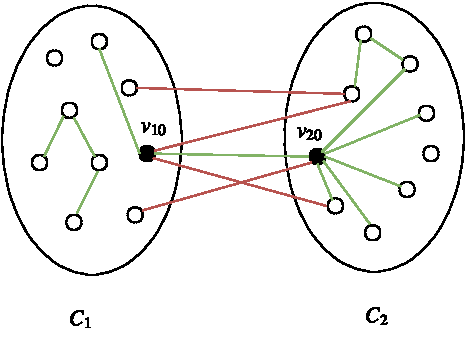
\includegraphics{./img/bipartite.pdf}
% \caption{20 points in 2 clusters. $C_1$ and $C_2$ are "natural" clusters}
% \label{fig:1}
% \end{figure}

%Now consider a case where instead of $20 = 2 \times 10$ points,
%This is denoted the "natural" clustering which has a cost of $0$ and its components are known as natural clusters.\\

\paragraph{Construction of $\NP$-hard PCC instances}
Construct a dataset having $2n$ points arranged into $n$ buckets, each having $2$ points. Pairs of points within the same bucket are separated by a $+$, while pairs of points in different buckets are separated by a $-$. From each of the $n$ buckets, one point is selected arbitrarily and labelled a \textit{bad vertex} of that bucket. The set of bad vertices are numbered in arbitrary order as $1,2,\dots,n$. An instance of PCC, denoted $\mathbf{I}_G$ is constructed from $G$ as follows: for every pair of vertices $i,j \in V$ if $(i,j) \in E$, then set $\sign (i,j)$ to $+$ from $-$. $B_i$ denotes the bucket corresponding to bad vertex $i$.

We are now ready to show the hardness reduction.

\begin{lemma}
Let $\opt (\mathbf{I}_G)$ denote the minimum set of vertices to remove from the instance $\mathbf{I}_G$ to make it perfectly clusterable. Then, $|\opt (\mathbf{I}_G )| = |VC(G)|$, where $VC(G)$ is the minimum vertex cover of the graph $G$.
\end{lemma}
%Observe that the optimal solution to this correlation clustering instance places each bucket of points in an independent cluster.

In order to prove this statement, we claim that (i) $|\opt (\mathbf{I}_G) \le |VC(G)|$ and (ii) $|\opt (\mathbf{I}_G) \ge |VC(G)|$.
\begin{claim}
$|\opt (\mathbf{I}_G)| \le |VC(G)|$
\end{claim}
Recall that $\opt (\mathbf{I}_G)$ is the minimum set of vertices removing which the instance $\mathbf{I}_G$ is perfectly clusterable. In order to show an upper bound to $\opt (\mathbf{I}_G)$, it is sufficient to fix an explicit clustering and compute the minimum number of vertices that need to be removed from this clustering to bring its cost to $0$.

So, consider a clustering, $\mathcal{C}$ where each bucket is placed in an independent cluster. Then, the set of mis-classified edges are nothing but the set of $+$ edges between bad vertices. Recall that by the labelling of vertices in $G$, $VC(G)$ can be represented as a subset of $\{1,2,\dots,n\}$. Removing the vertices labelled $VC(G)$ from the instance $\mathbf{I}_G$ is guaranteed to reduce the cost of the clustering $\mathcal{C}$ to $0$, since at least one end point of every mis-classified edge is removed (by definition of vertex cover).

\begin{claim} \label{lemma:01321923}
$|\opt (\mathbf{I}_G)| \ge |VC(G)|$
\end{claim}
In order to prove this lemma, we begin with the following claim.

\begin{claim}
For every pair of bad vertices $(i,j)$, such that $\sign (i,j) = +$, at least one vertex must be removed from either $B_i$ or $B_j$ for the cost of any clustering to be $0$.    
\end{claim}
\begin{proof}
Let the 2 points in $B_i$ be denoted $i$ and $i_1$ and likewise for $B_j$, $j$ and $j_1$. Then, for the cost of any clustering to be $0$, all the 4 points must be in the same cluster, since $\sign(i_1,i) = \sign (i,j) = \sign(j,j_1) = +$. However, even in this case $\sign(i_1,j_1) = -$ which incurs a cost of at least $1$.
\end{proof}

In order to prove Lemma \ref{lemma:01321923}, construct a graph $H$, where every node corresponds to a bucket and nodes corresponding to $B_i,B_j$ have an edge between them if $\sign (i,j) = +$. Consider the minimum set of nodes $S_{\min}$, such that every pair of buckets separated by a $+$ have at least one vertex chosen. In other words, every edge $(i,j)$ in $H$ has at least one point chosen from either $B_i$ or $B_j$. Any set of $B_i$ that have at least one vertex chosen from them cannot be less than $|VC(H)|$, by definition of minimum vertex cover. Therefore,
\begin{equation*}
	|S_{\min}| \ge |VC(H)| = |VC(G)|.
\end{equation*}
where the last equality follows from the fact that $H$ is isomorphic to $G$.

% \begin{figure}[ht]
% \centering
% 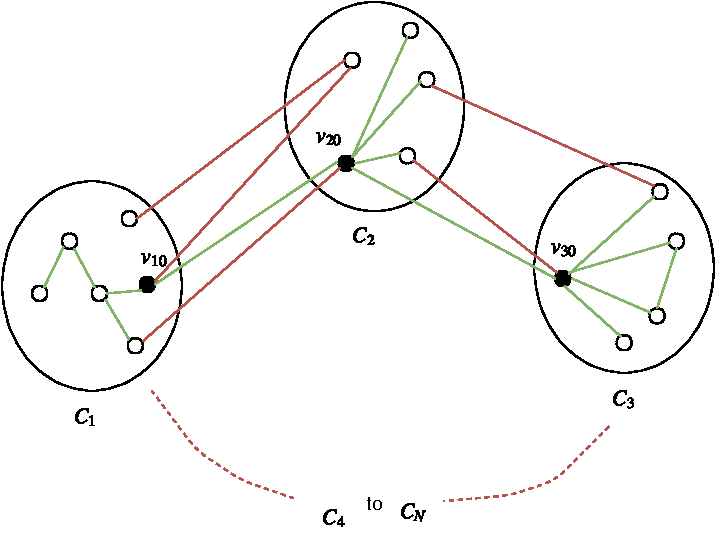
\includegraphics{./img/multipartite.pdf}
% \caption{$n$ points with $N$ "natural" clusters - $C_1, C_2, \dots, C_N$}
% \label{fig:2}
% \end{figure}

Therefore, $\mathbf{I}_G$ optimally, outputs $|VC(G)|$. Therefore, Robust Correlation Clustering is NP-hard.

%In robust correlation clustering, we need to remove $m$ vertices such that the cost of the natural (optimal) clustering on the resultant subgraph is minimized. The choice of these vertices must be from the set of bad vertices, since other vertices do not reduce the clustering cost. Consider an unweighted graph $G'$ defined on the $N$ bad vertices such that if two bad vertices are similar, they have an edge between them and if they are dissimilar, there is no edge between them. This graph captures the $- \to +$ swaps made previously. The goal is to then pick $m$ vertices from this graph such that their removal results in the least number of edges left over. This problem is as hard as vertex cover, since if I can solve it, I can decide if there is a vertex cover of size $m$ (if it is a vertex cover, the number of remaining edges will be $0$. If it is not, the number of edges will be $> 0$). Therefore, it is NP-hard to solve $m$-robust correlation clustering.

\end{proof}

%\input qns
%\input{combo}

%\newpage
%\listoftodos

\end{document}






































